\documentclass[12pt,oneside]{article}

%% --- encoding the docs------------------
\usepackage[T1]{fontenc}
\usepackage[utf8]{inputenc}


%--- Math environments-------------------
\usepackage{amsmath, amssymb}

%%--- Miscellaneous Environments ---------
\usepackage{xcolor} % for color
\usepackage{bold-extra} % To use sc as well as bf together
\usepackage{graphicx} % to insert figure
\usepackage{longtable} % to use table over the pages 


%%----Page Layout ------------
\usepackage[lmargin=3cm, rmargin=2cm, tmargin=3cm, bmargin=2cm]{geometry}

%%---- Header and Footer-----
\usepackage{fancyhdr}
\fancyhf{} 
\fancyhead[R]{\textnormal{\nouppercase\leftmark}}
\fancyfoot[C]{\thepage}
%%---- Line spacing ---------
\renewcommand{\baselinestretch}{2}

%%---- Font ----------
\usepackage{times} % Time new roman font

\usepackage{lipsum}


\newenvironment{preface}[1]{
	\newpage \thispagestyle{empty}
	   \addcontentsline{toc}{section}{#1}
	\begin{center}\vspace*{1.5cm} {\Large\sf \bfseries #1} \vspace{0.5cm}\end{center}
}{}

\newenvironment{certificate}{
	\newpage \thispagestyle{empty}
	\addcontentsline{toc}{section}{Certificate}
	\begin{center}
		
\includegraphics[scale=.6]{img/smit-logo}\\[-1.5em]
		{\color{orange}\bf (Constituent College of Sikkim Manipal University)}\\[1em]
		{\Large\sf  \sc \textbf{\underline{CERTIFICATE}}}
	\end{center}
}{}

%%--- for TOC-------------------------
\renewcommand{\contentsname}{\centering\Large\sf \bfseries Contents}
\renewcommand{\listfigurename}{\centering\Large\sf \bfseries LIst of Figures}
\renewcommand{\listtablename}{\centering\Large\sf \bfseries LIst of Tables}


%%% -------- Theorem Environments --------
\usepackage{amsthm}
\theoremstyle{definition}
\newtheorem{definition}{Definition}[section]
\newtheorem{example}[definition]{Example}
\newtheorem{problem}[definition]{Problem}

\theoremstyle{remark}
\newtheorem{remark}[definition]{Remark}

\theoremstyle{theorem}
\newtheorem{theorem}[definition]{Theorem}
\newtheorem{proposition}[definition]{Proposition}
\newtheorem{lemma}[definition]{Lemma}
\newtheorem{corollary}[definition]{Corollary}
\newtheorem{conjecture}[definition]{Conjecture}

\renewcommand\qedsymbol{$\blacksquare$}


%%%--- Hyperref----------------------------
\usepackage{hyperref}
\hypersetup{
colorlinks = true,
linkcolor=black,
citecolor=blue!50!black
}



%%--------- Student related settings---------
\newcommand{\thesistitle}{Title of the Project}
\newcommand{\studentname}{Student Name}
\newcommand{\regno}{xxxxxxxx}

%%--------- Guide related settings ----------
\newcommand{\guidename}{Dr.\,Guide Name}
\newcommand{\guidedesignation}{Assistant Professor}

%%--------- Course related settings---------
\newcommand{\degree}{Master of Science}
\newcommand{\coursename}{Mathematics}
\newcommand{\courseduration}{2018-2020}
\newcommand{\submissiondate}{July 2020}

%%--------- Department & Institute  related settings---------
\newcommand{\hodname}{Prof. (Dr.) Anjan Raychaudhuri}
\newcommand{\department}{Department of Mathematics}
\newcommand{\institute}{Sikkim Manipal Insitute of Technology}
\newcommand{\university}{Sikkim Manipal University}

\begin{document}

\pagenumbering{roman}
\begin{titlepage}
\centering
\large 
\vspace*{-2\baselineskip}

\includegraphics[scale=.6]{img/smit-logo}\\[-1.5em]

{\color{orange}\bf (Constituent College of Sikkim Manipal University)}\\[1em]

\rule{\linewidth}{2pt}
{\Huge\textbf{\thesistitle}}
\rule{\linewidth}{4pt}

{A dissertation submitted by\\
	
	{\bf  \studentname}\\
	
	(Reg. No. \regno)\\[\baselineskip]
	
	in partial fulfilment\\
	\baselineskip=18pt for the award of the Degree of \\
	
	{\bf \degree}\\
	
	(\coursename)\\[2\baselineskip]
	
	\baselineskip=18pt 	under the guidance of \\
	\baselineskip=18pt \textbf{\guidename}\\
	\baselineskip=18pt 	\guidedesignation
	
	\vfill

	\textsc{\department}\\
	
	\textsc{\institute}\\
	\textsc{Sikkim Manipal University}
	\submissiondate}
	\vspace{1em}

\end{titlepage}
\begin{preface}{Declaration}
I do hereby declare that the work contained in this dissertation entitled ``\textbf{\textsc{\thesistitle}}'' 
has done by me, under the supervision of {\guidename},
{\guidedesignation}, {\department}, SMIT in partial fulfillment
for the award of the degree of Master of Science and
this work has not been submitted elsewhere for a degree or diploma.

\vspace*{1in}
\begin{minipage}[t]{0.4\textwidth}
\baselineskip=18pt Place: Majitar \\
\baselineskip=18pt Date: 
\end{minipage}
\begin{minipage}[t]{0.5\textwidth}
\begin{center}
    {\bf    \studentname}\\
   \baselineskip=18pt  Reg No. \regno\\
    \baselineskip=18pt  \department\\
   \baselineskip=18pt  \institute\\
   \baselineskip=18pt  India.
\end{center}
\end{minipage}
\end{preface}
\begin{certificate}
This is to certify that the  dissertation entitled
\begin{center}
``{\large \textsc{\textbf{\thesistitle}}}''

submitted by

\textbf{\large \studentname}\\
\baselineskip=18pt  Reg. No. \regno
\end{center}
     \noindent in partial fulfilment for the award of the degree in \degree\, (\coursename) from \institute\, during \courseduration\, is a record of bona-fide work carried out under the supervision and guidance of \guidename, \guidedesignation, \department, \institute. The matter embodied in this dissertation has not been submitted to any other university for the award of any degree or diploma.

\vspace*{2cm}
\noindent

\begin{minipage}[t]{0.45\textwidth}
	\baselineskip=18pt
	\centering
    \noindent {\bf \hodname }\\
    Head of the Department\\
    \department\\
    \institute\\ 
    \university\\
     India
\end{minipage}
\hspace*{.1\textwidth}
 \begin{minipage}[t]{0.45\textwidth}
 	\baselineskip=18pt
 	\centering
 \noindent {\bf \guidename}\\
    \guidedesignation\\
    \department\\
    \institute\\
     \university\\
      India
\end{minipage}
\end{certificate} 
\begin{preface}{Acknowledgements}
\lipsum[2-5]


\vspace{1in}
\noindent
\begin{minipage}[t]{0.3\textwidth}
\baselineskip=18pt
Place: \\
Date: 
\end{minipage}
\begin{minipage}[t]{0.65\textwidth}
\begin{flushright}
\baselineskip=18pt
    {\bf  \studentname}\\
    \institute,  India\\
\end{flushright}
\end{minipage}

\end{preface} % Acknowledgements
\begin{preface}{Abstract}

\lipsum[2]

\end{preface} % abstract


\clearpage 
\tableofcontents
\clearpage 

\listoffigures % You may comment it if you dont have any figures
\clearpage  % You may comment it if you dont have any figures

\listoftables  % You may comment it if you dont have any tables
\clearpage % You may comment it if you dont have any tables

\begin{preface}{List of Symbols}
\begin{longtable}{lcl}
$\mathbb{R}$ & : & Set of all real numbers \\
$\mathbb{R}^{m\times n}$ & : & Set of all $m\times n$ matrices over $\mathbb{R}$
\end{longtable}
\end{preface}
\clearpage 

\pagestyle{fancy}
\pagenumbering{arabic}

%%--- Main-content------
\section{Introduction}

Ut vehicula sollicitudin vulputate. Morbi sit amet mi nisi. Sed gravida porta dapibus. Nam in ligula fermentum, vehicula justo congue, volutpat odio. In et ornare diam. Nunc molestie scelerisque faucibus. Fusce ut nunc volutpat, sodales elit ut, placerat risus. Fusce ac erat ipsum. Donec in magna sit amet justo pulvinar tincidunt. Mauris eleifend, mauris non tincidunt rhoncus, nulla urna viverra eros, vel egestas metus justo sed nisl.

\begin{definition}[Fibration]
A \emph{fibration} is a mapping between two topological spaces that has the homotopy lifting property for every space $X$.\end{definition}

Mauris quis egestas massa. Integer ut rutrum nibh, quis vulputate lectus. Nulla dignissim, tortor eu luctus commodo, diam lectus hendrerit ipsum, a convallis dolor velit eu diam. Sed sit amet erat urna. Maecenas sit amet facilisis augue. Ut a rhoncus diam, ut euismod velit. Pellentesque fringilla euismod risus. Maecenas vitae lacinia augue. Etiam eu mollis nulla, eu facilisis enim. Quisque ullamcorper ultricies risus non ultrices. Aliquam erat volutpat. Praesent sed velit iaculis, commodo sem ac, faucibus augue.
\begin{equation}\label{eq:something}
\left[  \frac{ N } { \left( \frac{L}{p} \right)  - (m+n) }  \right]
\end{equation}
In the \autoref{eq:something}, we have discussed something
\begin{equation}
\binom{n}{k} = \frac{n!}{k!(n-k)!}
\end{equation}

\subsection{Some subsection}
 Sed sit amet erat urna. Maecenas sit amet facilisis augue. Ut a rhoncus diam, ut euismod velit. Pellentesque fringilla euismod risus. Maecenas vitae lacinia augue. Etiam eu mollis nulla, eu facilisis enim. Quisque ullamcorper ultricies risus non ultrices. Aliquam erat volutpat. Praesent sed velit iaculis, commodo sem ac, faucibus augue.
 \begin{theorem}[]
 	content...
 \end{theorem}


\section{Literature Review}

A matrix for example $\begin{pmatrix}
	1 & 0\\
	0 & 1
\end{pmatrix}$ can be also used in the document... Integer dui leo, fringilla eu ultrices tincidunt, sollicitudin nec sapien. Cras nec ligula non sem blandit sollicitudin sit amet vitae leo. Aenean accumsan ligula tincidunt, consectetur magna consectetur, porttitor enim. Nam quis volutpat ex. Cras sit amet finibus velit. Maecenas bibendum scelerisque lectus, at elementum urna faucibus ut. Suspendisse tempor tellus in lacus feugiat pretium. Nulla nec eros faucibus, facilisis mauris vitae, gravida nunc.

\subsection{Some subsection}
\lipsum[10]
\begin{lemma}
	Given two line segments whose lengths are $a$ and $b$ respectively there 
	is a real number $r$ such that $b=ra$.
\end{lemma}

\begin{proof}
	To prove it by contradiction try and assume that the statement is false,
	proceed from there and at some point you will arrive to a contradiction.
	\begin{align*}
	f(x) &= x^2\\
	g(x) &= \frac{1}{x}\\
	F(x) &= \int^a_b \frac{1}{3}x^3
	\end{align*}
\end{proof}
Cras sit amet finibus velit. Maecenas bibendum scelerisque lectus, at elementum urna faucibus ut. Suspendisse tempor tellus in lacus feugiat pretium. Nulla nec eros faucibus, facilisis mauris vitae, gravida nunc.

\subsection{Some subsection}
 Donec luctus volutpat orci. Aliquam purus erat, suscipit eget aliquam ut, maximus vel enim. Quisque semper imperdiet tellus in scelerisque. Nunc ornare non odio ut porta. Suspendisse dapibus vitae ante at condimentum. Nullam vel efficitur sapien. Nunc urna mi, luctus ut magna nec, viverra faucibus quam. In vehicula velit nec diam scelerisque pulvinar.
 
 \begin{theorem}
 	Given two line segments whose lengths are $a$ and $b$ respectively there 
 	is a real number $r$ such that $b=ra$.
 \end{theorem}
 
 \begin{proof}
 	To prove it by contradiction try and assume that the statement is false,
 	proceed from there and at some point you will arrive to a contradiction.
 	\begin{equation*}
 	 f(x) = \sum_{i=0}^{n} \frac{a_i}{1+x} 
 	\end{equation*}
 \end{proof}

\section{Main Section}
\lipsum[4] \cite{horn1985}
\subsection{Inserting Figures}
Sed dignissim nec magna a eleifend. Fusce vel ex sed tellus accumsan scelerisque. Vestibulum sed odio sed turpis fringilla accumsan non sed erat. Etiam dapibus rhoncus velit at vestibulum. Suspendisse potenti. Praesent vitae vulputate purus. Quisque quis porttitor sem. Aenean ipsum nisl, consectetur eu condimentum ac, porta at eros.\cite{jeff06}
\begin{figure}[htb!]
\centering
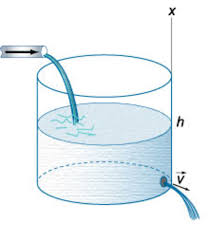
\includegraphics[scale=.75]{img/fluid-flow}
\caption{Fluid flow from a vessel}
\label{fig:fluid_flow}
\end{figure}
 Fusce vel ex sed tellus accumsan scelerisque. Vestibulum sed odio sed turpis fringilla accumsan non sed erat. Etiam dapibus rhoncus velit at vestibulum.

\subsection{Inserting Tables}
Cras nec ligula non sem blandit sollicitudin sit amet vitae leo. Aenean accumsan ligula tincidunt, consectetur magna consectetur, porttitor enim \cite{kir86}. Nam quis volutpat ex. Cras sit amet finibus velit. Maecenas bibendum scelerisque lectus, at elementum urna faucibus ut. Suspendisse tempor tellus in lacus feugiat pretium. Nulla nec eros faucibus, facilisis mauris vitae, gravida nunc.
\begin{table}[h!]
\centering
		\begin{tabular}{l|c|r} 
			\hline 
			$\alpha$ & $\beta$ & $\gamma$ \\
			\hline
			1 & 1110.1 & a\\
			2 & 10.1 & b\\
			3 & 23.113231 & Some\\ \hline 
		\end{tabular}
\caption{Table of values}
\label{tab:values}
\end{table}


\subsection{Some more subsection}
Ut a rhoncus diam, ut euismod velit. Pellentesque fringilla euismod risus. Maecenas vitae lacinia augue. Etiam eu mollis nulla, eu facilisis enim. Quisque ullamcorper ultricies risus non ultrices. Aliquam erat volutpat. Praesent sed velit iaculis, commodo sem ac, faucibus augue.\cite{rbb2010}\\
\section{Conclusion}
Sed volutpat, libero in mollis maximus, lorem nibh dictum velit, a aliquam justo risus ac dui. In ullamcorper, nulla nec interdum luctus, tortor est aliquet est, id scelerisque mauris odio ac mauris. Donec luctus volutpat orci. Aliquam purus erat, suscipit eget aliquam ut, maximus vel enim. Quisque semper imperdiet tellus in scelerisque. Nunc ornare non odio ut porta. Suspendisse dapibus vitae ante at condimentum. Nullam vel efficitur sapien. Nunc urna mi, luctus ut magna nec, viverra faucibus quam. In vehicula velit nec diam scelerisque pulvinar.



%%%--- References Section------
\addcontentsline{toc}{section}{\bf References}
\bibliographystyle{plain}
\bibliography{refs/bibliography}

\end{document}